% Very simple template for lab reports. Most common packages are already included.
\documentclass[a4paper, 11pt]{article}
\usepackage[utf8]{inputenc} % Change according your file encoding
\usepackage{graphicx}
\usepackage{url}

%opening
\title{Rudy: a small web server}
\author{Chrysoula Dikonimaki}
\date{\today{}}

\begin{document}

\maketitle

\section{Introduction}

This report describes Rudy, a small web server implemented in Erlang using the gen\_tcp library. Also, this report provides the results of server's performance evaluation as well as bonus improvements.

\section{Main problems and solutions}

Our server receives HTTP GET requests from a client (e.g. a browser) and replies with HTTP 200 OK message. In order to be able to achieve this, our server does the following steps:
\begin{enumerate}
  \item Opens a listening socket (init).
  \item When a request comes, the server accepts it and now we have a connection opened with the client (handler).
  \item Finally, the server reads the input (request), parses it (http:parse\_request) and replies (reply).
\end{enumerate}
The steps described above is the happy path. I added the necessary lines of code to complete the server implementation. 

\section{Tests}
First of all, I changed the bench function in the test.erl file to take as an input a number M which should be the number of requests that will be sent.
\subsection{Test 1}
\label{test1}
In order to evaluate Rudy while simulating one machine, I created a file called test1.erl and I implemented a function called run\_bench which gets as input the host, the port, a number N which is the number of times the bench function will be called and M which is the number of requests that will be sent and returns the average time in seconds. 
\subsection{Test 2}
\label{test2}
In order to evaluate Rudy while simulating  multiple machines I created a file called test2.erl and I implemented a function called run\_bench which takes as input the id of the process which calls it (e.g. self())  the host, the port, a number N which is the number of machines and M which is the number of requests will be sent and returns the average time in seconds. 

\section{Improvements}

\subsection{Increasing throughput}
The improvements implemented were two. The first one is the Version 1 (rudy\_v1.erl). At this version of the server, each request is handled concurrently so one new process is created for each new request.
The second improvement is Version 2 (rudy\_v2). At this version, a pool of processes is created when the server starts for the first time which means that all processes are waiting at the same port. Thus, when a request comes one of these processes handles it.

\subsection{Deliver files}
In order to deliver files I created a directory called “data” which contains some html files. Our server will serve the files under this directory. So if we try to access the “http://localhost:8080/data/index.html” the content of the “data/index.html” file will be retrieved. 
The implementation is inside the “rudy\_v3.erl” file. The main changes are two. The first one is that I added the function parse\_uri which takes as input the URI and returns the path and the file name. For example, for the “http://localhost:8080/data/index.html” it returns “/data” and “index.html”. Moreover, I changed the reply function to parse the URI, read the file if it exists and return it to the browser. 


\section{Evaluation}
All figures have been created with Python and the matplotlib library.

\subsection{Simulating one machine}
I ran the  run\_bench function described in \ref{test1} setting M=[1,10,100,200] and N=10, one time with the artificial delay and one time without  it. The results are shown in Figure \ref{fig:results1}.

\begin{figure}
  \begin{center}
    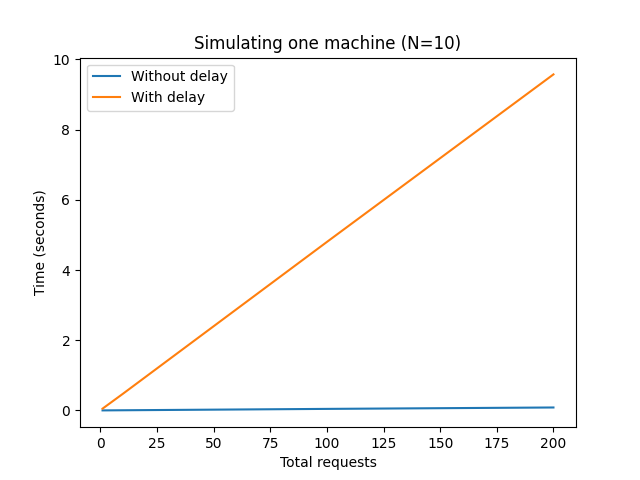
\includegraphics[scale=0.4]{result1.png}
    \caption{Simulating one machine}
    \label{fig:results1}
  \end{center}
\end{figure}

As we can see the artificial delay is significant and reduces the number of requests per second our server can handle (increases dramatically the time it takes to send the requests).  

\subsection{Simulating multiple machines}
I ran the  run\_bench function described in \ref{test2} for each version of the server setting N=[10, 20, 30, 40] and M=100. The results are shown in Figure \ref{fig:results1}.

\begin{figure}
  \begin{center}
    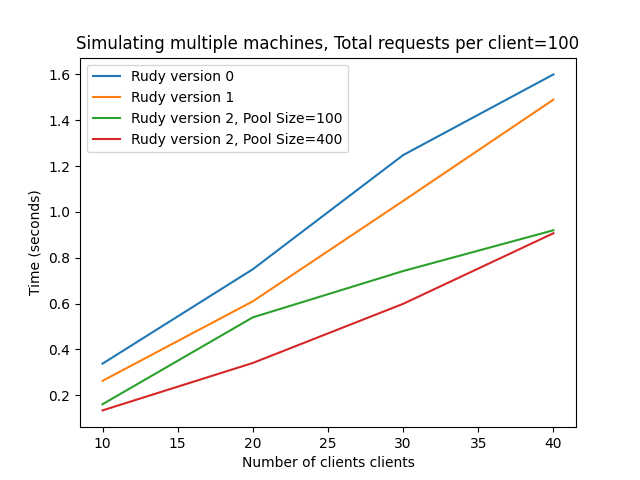
\includegraphics[scale=0.4]{result2.png}
    \caption{Simulating multiple machines}
    \label{fig:results2}
  \end{center}
\end{figure}
It is clear that having a pool with multiple processes running takes less time than all the other cases, so the version 3 is the best.

\section{Conclusions}
This homework was a good introduction to Erlang programming and to the HTTP protocol.
\end{document}
